\chapter{Methodology}

Text to speech (TTS) synthesis is the process of transformation of data from textual form into voice output. This process is divided in two sub modules. One module performs analysis and preprocessing of data and other transforms processed data into sound signals. This is shown in \ref{fig:TTS Sub Modules}

\begin{figure}[hp]
  \centering
  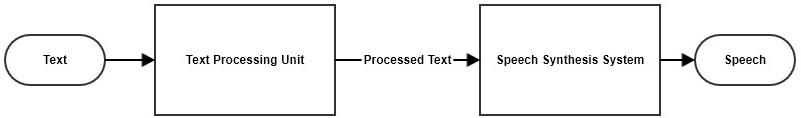
\includegraphics[width=\linewidth]{images/tts_flow_dg.jpg}
  \caption{TTS Sub Modules}
  \label{fig:TTS Sub Modules}
\end{figure}

\section{Text Processing Unit}
Text processing unit is responsible for processing of text before it is sent to speech synthesis system. It finds numbers, dates and time in input data and converts it into format acceptable by speech synthesizer. This module consists of following sub modules.

\begin{enumerate}
  \item Special Character Processor
  \item Semantic Tagger  
  \item Text Generator
  \item Text Formatter 
\end{enumerate}

\subsection{Special Character Processor}

Raw text may contain special characters such as punctuation marks. These characters help to understand context of a word but 
are not converted into sounds. We remove all such characters from text before further processing. 
Another processing which is done is conversion of all arabic numerals like \textarabic{١}, \textarabic{٢} and \textarabic{٣} into their corresponding 
characters like 1, 2 and 3 because it is easy to further process text after it has been converted into same type of numerals.

\subsection{Semantic Tagger}
The purpose of Semantic Tagger is to identify numbers, dates and time from input data and give them proper tags. 
All numbers in input data are converted into arabic numerals of type 1, 2 and 3 in previous step. 
There can be multiple form of numbers, dates and time. These forms are explained below.


\begin{enumerate}    
  \item Dates in following format

  \begin{enumerate}[label=\alph*.]
    \item 12/11/2018 or 12/11/18 with different separators like \enquote{/} or \enquote{-} or \enquote{.}
    \item \texturdu{12 دسمبر 2012}
    \item \texturdu{12 دسمبر}
  \end{enumerate}
  \item Number in following format
  \begin{enumerate}[label=\alph*.]
    \item Whole Numbers such as 123
    \item Floating point numbers such as 12.3
  \end{enumerate}

  \item Time in following format

  \begin{enumerate}[label=\alph*.]
    \item 12:12
    \item 12:12:12
  \end{enumerate}
\end{enumerate}


In table \ref{table:semantic_tagger_regex}, regex used for identification of these numbers, dates and time are shown.

\begin{table}[]
\centering
\resizebox{\textwidth}{!}{%
\begin{tabular}{|c|c|c|}
\hline
\textbf{Regex} & \textbf{Type} & \textbf{Example} \\ \hline
(\textbackslash{}d+(?:\textbackslash{}.\textbackslash{}d+)?) & Integer or Floating point number & 123 or 12.312 \\ \hline
\textbackslash{}d\{1,2\}:\textbackslash{}d\{1,2\}(?::\textbackslash{}d\{1,2\})? & Time with or without seconds & 5:12 or 5:12:10 \\ \hline
\textbackslash{}d\{1,4\}{[}./-{]}\textbackslash{}d\{1,4\}{[}./-{]}\textbackslash{}d\{1,4\} & Date with separator like \enquote{/} or \enquote{-} or \enquote{.} & 12-10-2018 or 12/10/18 \\ \hline
\%s \textbackslash{}d\{4\} & Dates with month name in Urdu. This is checked by replacing \%s with each month name separately. & \texturdu{12 دسمبر} \\ \hline
\end{tabular}%
}
\caption{Regular Expression for Semantic Tagger}
\label{table:semantic_tagger_regex}
\end{table}

\subsection{Text Generator}
Semantic tagger will return all numbers, dates and time from text with each one marked as date/time/number. Text generator part will take each word and generates Urdu text according to its tagging. Each tagged number is handled by specific text converter. These converters are listed below.

\begin{enumerate}
  \item Number to text converter
  \item Date to text converter 
  \item Time to text converter
\end{enumerate}

\subsubsection{Number to Text Converter}
This unit will deal with whole numbers, fractional numbers and decimal numbers. In table \ref{table:no_conversion_example}, example conversions are shown. 

\begin{table}[]
\centering
\begin{tabular}{|c|c|}
\hline
\textbf{Word} & \textbf{Converted Text}                          \\ \hline
123           & \texturdu{ایک سو تئیس}                                     \\ \hline
1231          & \texturdu{ایک ہزار دو سو اکتیس}                            \\ \hline
123.1234      & \texturdu{ایک سو تئیس اعشاریہ ایک دو تین}                   \\ \hline
12345         & \texturdu{بارہ ھزار تین سو پینتالیس}                        \\ \hline
1234567       & \texturdu{بارہ لاکھ چونتیس ھزار پانچ سو ستاسٹھ}             \\ \hline
987654321     & \texturdu{اٹھانوے کروڑ  چھہتر لاکھ   چون ھزار تین سو اکیس}  \\ \hline
143.159874    & \texturdu{ایک سو تینتالیس  اعشاریہ ایک پانچ نو آٹھ سات چار} \\ \hline
\end{tabular}
\caption{Number Conversion example}
\label{table:no_conversion_example}
\end{table}

Different process is performed in order to handle fractional and integer parts of floating point numbers. The algorithm for integral number is described below.

\begin{minted}[mathescape,
               breaklines, 
               numbersep=5pt,
               gobble=1,
               frame=lines,
               framesep=1mm]{python}
  def get_factors(number):
    factored_integer_list = [100000000000, 1000000000, 10000000, 100000, 1000, 100]
    factored_number = []
    for factor in factored_integer_list:
        If factor > number and number != 0:
            factored_number.append(number/factor)
            factored_number.append(factor)
            number = number % factor  
    If number != 0:
        factored_number.append(number)
    return factored_number

\end{minted}

This algo will return list of factored numbers and factors. For 1213, the result of this algorithm will be 
[1, 1000, 2, 100, 13]. The integer to Urdu mapping for number 0 to 100 and number like 1000, 100000 etc are 
stored in CSV file. The factored number list will then be converted into text by using integer to Urdu mapping. 
In table \ref{table:number_mapping}, Urdu mapping of each possible factor is listed. Each number in fractional 
part of floating pointing number is replaced by their respective mapping from above list. 
Both the mappings of integral and fractional part of number are then joined to get
complete text of input number. This module is very important module as it is also used in date and time conversion.  

\subsubsection{Date to Text Converter}

The unit deals with date in following formats

\begin{itemize}
  \item 12/12/2012
  \item 12/12/12
  \item 12.12.2012
  \item 12.12.12
  \item 12-12-2012
  \item 12-12-12
  \item \texturdu{12 دسمبر 2012}
\end{enumerate}

All dates will be converted into common format e.g. \texturdu{ بارہ دسمبر دو ہزار بارہ}. Some example conversions are shown in table \ref{table:example_of_date_conversions}.

\begin{table}[]
\centering
\begin{tabular}{|c|c|}
\hline
\textbf{Date} & \textbf{Converted Text}            \\ \hline
12/10/15      & \texturdu{دس دسمبر  دو ھزار پندرہ} \\ \hline
12.10.15      & \texturdu{دس دسمبر  دو ھزار پندرہ} \\ \hline
12-10-15      & \texturdu{دس دسمبر  دو ھزار پندرہ} \\ \hline
12.10.1989    & \texturdu{دس دسمبر انیس سو نواسی}  \\ \hline
\end{tabular}
\caption{Example Date Conversions}
\label{table:example_of_date_conversions}
\end{table}

The word tagged as date is first processed to get year, month and day of the month. Day and year are then passed to number to text converter and month is 
converted to its corresponding mapping. This mapping is saved in CSV file. This is shown in table \ref{table:month_mapping}. 
In Urdu, in dates, we have different notation for year e.g. 1980 in number is spoken as \texturdu{ایک ھزار نو سو نواسی} (One thousand nine hundred and 
eighty nine) but in dates, it is spoken as \texturdu{انیس سو نواسی} 
(Nineteen hundred and eighty nine). This is also handled during the process of date to text conversion.


\subsubsection{Time to Text Converter}

Time can occur with seconds or without seconds in text. It is written in 1:11:12 or 1:12 format. All words tagged as time will be converted into text 
by separating hour, minutes and seconds from time. Each value will be converted into Urdu text by using number to text converter. All these values are 
combined to make complete time text. Table \ref{table:example_time_conversion} shows example conversions.

\begin{table}[]
\centering
\begin{tabular}{|c|c|}
\hline
\textbf{Time} & \textbf{Converted Text}                        \\ \hline
1:12:15       & \texturdu{ایک بج کر  بارہ منٹ اور پندرہ سیکنڈ} \\ \hline
7:45          & \texturdu{سات بج کر پینتالیس منٹ}              \\ \hline
\end{tabular}
\caption{Example Time Conversions}
\label{table:example_time_conversion}
\end{table}

\subsection{Text Formatter}
The purpose of formatter is to replace all number, dates and time with their corresponding Urdu text returned by Text generator. 
This process is performed in following order
\begin{enumerate}
  \item Word tagged as dates are replaced by their corresponding text
  \item Word tagged as time are replaced by their corresponding text
  \item Word tagged as number are replaced by their corresponding text. 
\end{enumerate}
The output of all above processes will be the text which will only contain Urdu text which can now pass to the speech synthesizer which will convert it to speech signals. 

\section{Speech Synthesis System}

\subsection{Tools}

Below are the tools used for the process of Speech Synthesis of Urdu.

\begin{enumerate}
  \item Speech Tools Library of Edinburg
  \item Festvox
  \item Speech Signal Processing Toolkit (SPTK)
  \item Festival
\end{enumerate}

\subsubsection{Speech Tools Library of Edinburg}
The Edinburgh Speech tools is collection of utilities used for speech processing. These utilities cover major tasks such that reading and 
writing speech waveforms, parameter files(F0 and LPC etc). The speech tools also include executable programs which can 
be used in user defined programs.


\subsubsection{Festvox}
Festvox is a tool which can be used to build synthetic voices. This includes scripts for building voice in other languages.

\subsubsection{ Speech Signal Processing Toolkit (SPTK)}
As name suggests, this tool is for processing speech signals in UNIX systems. 

\subsubsection{Festival}

Festival \cite{thefestivalspeechsynthesissystem} is a speech synthesis system which is developed in Centre for Speech Technology Research (CSTR) \cite{centreforspeechtechnologyresearch}. It is a multi-platform framework for building speech synthesis system. This system is outlined so that it tends to be utilized for following purposes

\begin{enumerate}
  \item Improvement in speech synthesis system
  \item Developing speech synthesis applications
\end{enumerate}

One of the main thing that makes Festival very useful is scripting language which is based upon Scheme programming language. This can be used to manage parameters and flow of  control in Festival. 

\subsection{Process}

The process of speech synthesis is based on statistical parametric speech synthesis. The statistical parametric speech synthesis system is based on models like HMM or DNN in which recorded speech is used to train model. In this method, speech is elaborated with parameters which are defined by statistics. This is why it is called as statistical parametric speech synthesis. 

In CLUSTERGEN statistical parametric speech synthesis, model is trained and used for synthesis in Festival Speech Synthesis system. 

\subsubsection{Preparing Data}

For training purpose, Phonetically Rich Urdu Speech Corpus \cite{urdu_corpus} is used. This data consists of recordings of 708 phonetically rich sentences, 
10,101 tokens with 5,656 unique words. Total duration of recording is 70 minutes.

\subsubsection{Data Labeling}
Data is labeled in specific format which is required by FestVox for training purpose. The is labeled in following format.
\\ \\
( c1 "\texturdu{نیلم نے سالگرہ پر ہیڈ سیسموگراف اسود قریشی کے ماتھے پر اینٹھن اور غم کی آتشیں رو محسوس کی}" )

Where c1 is the name of recording file and text between quotation marks is corresponding label of that recording.

\subsubsection{Training Data}

The whole data is further divided in 10:1 ratio in training and test set respectively.


\subsubsection{Urdu to Hindi Transliteration}

The underlying system of Urdu TTS is Hindi TTS system. So all the alphabets are mapped in their corresponding Hindi alphabets. 
In this way, text is first converted into corresponding Hindi text using that mapping and then it is converted into sound. 
Mapping of each Urdu word with Hindi in this system is shown in table \ref{table:hindi_to_urdu}.

\subsubsection{Data Labeling}

The first stage of training is to label speech database using HMM labeler. We are using EHMM labeler which is provided in FestVox. In this process, Baum-Welch is used to train context dependent models. This labeler works in 8 steps. Prompt files are extracted from utterance structure of Festival.

\begin{itemize}
  \item Unique sequence of phones are extracted and stored.
  \item List of wav files is collected for feature extraction.
  \item From wav files, cepstral coefficients (LPCCs and MFCCs) are extracted.
  \item From cepstral coefficients, deltas and delta-delta features are generated.
  \item By using generated features and wav files list, features vectors are modified.
  \item Phones list generated in step # 2 and wav file list is used to modify prompt list.
  \item Hidden Markov model is trained using Baum-Welsh algorithm till difference in the average likelihood is less than 0.001.
  \item Labels are generated according to training data.
  \item Integer indices of labels are converted into phone names
\end{enumerate}

\subsubsection{Building Utterance Structure}

Utterance is the essential building unit of Festival. It shows relation between bunch of items where each item relates to word, syllable or segment etc. Below are the some of the relations used in building utterance structure.

\begin{itemize}
  \item{\textbf{Text}:} It consists of strings to be processed and features of that string.
  \item{\textbf{Token}:} Token means each word in a sentence is separated by some language specific separator.
  \item{\textbf{Word}:} A small unit of speech which can be pronounced with the help of letter to sound rules of a language.
  \item{\textbf{Phrase}:} Phrase means group of words forming a part of a sentence.
  \item{\textbf{Syllable}:} Syllables are units which when combined with vowels form complete pronunciation of a word.
  \item{\textbf{Segment}:} Segment consists of list of phones.
  \item{\textbf{SylStructure}:} This is a tree structure which is formed with word, syllable and segment.
  \item{\textbf{IntEvent}:} These are array of syllable related intonation events.
  \item{\textbf{Intonation}:} Intonation means rise and fall in speech signals.
\end{itemize}


\subsubsection{Coefficient Extraction}
Coefficient extraction is the process of extracting parameters like F0, mcep and voicing coefficients using SPTK. This is done by 
generating F0 and mcep coefficient. These parameters are then combined to make final parameter files. 
This is a lengthy process which can take lot of time depending on size of training data.

\subsubsection{Building the Model}

All the data generated above is used to train and build HMM-state duration model. This process works in following steps.

\begin{enumerate}
  \item Statenames Generation
  \item Parametric Model generation
  \item Duration model generation for statenames
\end{enumerate}

This resulting model can be used to perform TTS synthesis process.
